
\section{SQS}
\label{sec:sqs}

\subsection{Introduction}
In this section we describe our work on the static code analysis of the bitwalker code provided in \href{https://github.com/openETCS/validation/tree/master/Artifacts/Subset-026-7_XML/Subset026_7/Bitwalker}{[validation repository]}

Our aim is to discover programing errors, obtain code metrics (lines of code, lines of code/lines of comments, cyclomatic complexity, class inherance tree and others) and verify some subset of rules defined in the MISRA C Standard.

The code metrics help understanding the complexity of the code and can lead to code changes. For
example, the cyclomatic complexity or the number of paths, are a precise measure of the code complexity, and the more complex the code is, more likely it will contain masked bugs.

Five different static analysis tools have been used during the code verification activities in order to assess the quality of the results and ensure code quality.

Finally, according to the results obtained by using the tools, we will present some conclusions.

\subsection{Resource Standard Metrics -RSM- Results}
In this section we provide the results obtained with the RSM tool.

Resource Standard Metrics (RSM) is a source code metrics and quality analysis tool.

RSM provides standard metrics and a combination of features that allow to:
\begin{itemize}
\item Analyze source code for programming errors
\item Analyze source code for code style enforcement
\item Create an Inheritance tree from the code
\item Collect Source Code Metrics by the function, class, file, and project
\item Analyze Cyclomatic Complexity
\end{itemize}

Furthermore, RSM tool is mapped to the \href{http://msquaredtechnologies.com/m2rsm/docs/QualityStandards/MISRA_C_Mapping.htm}{[MISRA C]} Industry Standards which coverage is 40.16\% 


Besides, RSM has intrinsic quality notices and can be extended by the end user with User Defined Quality Notices using regular expressions to analyze code lines. 

The following table shows the intrinsic Quality Notices for language c that RSM tool checks.

{\footnotesize\sffamily\centering
  \begin{longtable}{||p{.45\textwidth}|p{.5\textwidth}||}
  \caption{Quality Notices}\\
    \hline\hline
    \hline\hline
    \endhead
    \hline\hline
    \endfoot
    \textbf{Quality Notice No. 1}

Emit a quality notice when the physical line length is greater than the specified number of characters.

Rationale:  \textcolor{red}{Reproducing source code on devices that are limited to 80 columns of text can cause the truncation of the line or wrap the line.  Wrapped source lines are difficult to read, thus creating weaker peer reviews of the source code}.
& \textbf{Quality Notice No. 2}

Emit a quality notice when the function name length is greater than the specified number of characters.  

Rationale:  \textcolor{red}{Long function names may be a portability issue especially when code has to be cross compiled onto embedded platforms.  This difficultly is typically seen with older hardware and operating systems.}
    \\
    \hline \textbf{Quality Notice No. 3}
    
Emit a quality notice when ellipsis '...' are identified within a functions parameter list thus enabling variable arguments.  

Rationale:  \textcolor{red}{Ellipsis create a variable argument list.  This type of design is found in C and C++.  It essentially breaks the type strict nature of C++ and should be avoided.}
 & \textbf{Quality Notice No. 4}
 
Emit a quality notice if there exists an assignment
operator '=' within a logical 'if' condition.

Rationale:  \textcolor{red}{An assignment within an "if" condition is likely a typographical error giving rise to a logic defect.  However, some programmers place compound statements into the "if" condition making the code difficult to read.}
    \\
    \hline \textbf{Quality Notice No. 5}
    
Emit a quality notice if there exists an assignment
operator '=' within a logical 'while' condition.

Rationale:  \textcolor{red}{An assignment within a "while" condition is likely a typographical error giving rise to a logic defect.  However, some programmers place compound statements into the "while" condition making the code difficult to read.}
 & \textbf{Quality Notice No. 6}
 
Emit a quality notice when a pre-decrement operator '--' is identified within the code.  

Rationale: \textcolor{red}{ The pre-decrement of a variable occurs before the remainder of the processing in the statement.  This can be difficult to comprehend or anticipate.  There are documented cases where the mathematical results vary between the result of macros when different code preprocessors expand the macros into a normal form.  Remember, there is no standard for the preprocessor, just the language.}
    \\
    \hline \textbf{Quality Notice No. 7}
    
Emit a quality notice when a pre-increment operator '++' is identified within the code.

Rationale:  \textcolor{red}{The pre-increment of a variable occurs before the remainder of the processing in the statement.  This can be difficult to comprehend or anticipate.  There are documented cases where the mathematical results vary between the result of macros when different code preprocessors expand the macros into a normal form.}  
& \textbf{Quality Notice No. 8}

Emit a quality notice when the 'realloc' function
is identified within the code.

Rationale:  \textcolor{red}{Using realloc can lead to latent memory leaks within your C or C++ code.  The call to realloc reassigns the pointer to the same memory address using a larger or smaller space.  However if realloc fails, a NULL pointer is returned.  No "free" was performed on the pointer so if you don't retain the pointer before the realloc call, a latent memory leak could occur.}
    \\
    \hline \textbf{Quality Notice No. 9}
    
Emit a quality notice when the 'goto' function
is identified within the code.

Rationale:  \textcolor{red}{The use of "goto" creates spaghetti code.  A "goto" can jump anywhere to the destination label.  This type of design breaks the "one in - one out" ideal of a function creating code which can be impossible to debug or maintain.}
 & \textbf{Quality Notice No. 10}
 
Emit a quality notice when the Non-ANSI function prototype is identified within the code.

Rationale:  \textcolor{red}{Older C code can be written in a style that does not use function prototypes of the function argument types.  This code will not compile on ANSI C and C++ compilers because of this type of weakness.  Identifying this condition can help assess whether code can be ported to a newer version of the language.}
    \\
    \hline \textbf{Quality Notice No. 11}
    
Emit a quality notice when open and closed brackets '[ ]' are not balance within a file.

Rationale:  \textcolor{red}{This type of error is always caught by the compiler as a syntax error.  However, a compiler can be told to ignore source code by using preprocessor directives like \#if ... \#endif.  This is a way to "comment" out large blocks of code.  However, the code still looks like operational code to the maintainer as it is not a comment.  Many hours can be wasted working on dead code.  This quality notice serves to warn you of this dead code that should be removed or converted to actual comment form.}
 & \textbf{Quality Notice No. 12}
 
Emit a quality notice when open and closed parenthesis '( )' are not balance within a file.

Rationale:  \textcolor{red}{This type of error is always caught by the compiler as a syntax error.  However, a compiler can be told to ignore source code by using preprocessor directives like \#if ... \#endif.  This is a way to "comment" out large blocks of code.  However, the code still looks like operational code to the maintainer as it is not a comment.  Many hours can be wasted working on dead code.  This quality notice serves to warn you of this dead code that should be removed or converted to actual comment form.}.
    \\
    \hline \textbf{Quality Notice No. 13}
    
Emit a quality notice when a 'switch' statement does not have a 'default' condition.

Rationale:  \textcolor{red}{A "switch" statement must always have a default condition or this logic construct is non-deterministic.  Generally the default condition should warn the user of an anomalous condition which was not anticipated by the programmer by the case clauses of the switch.}
 & \textbf{Quality Notice No. 14}
 
Emit a quality notice when there are more 'case' conditions than 'break', 'return' or 'fall through' comments.

Rationale:  \textcolor{red}{Many tools, including RSM, watch the use of "case" and "break" to insure that there is not an inadvertent fall through to the next case statement.  RSM requires the programmer to explicitly indicate in the source code via a "fall through" comment that the case was designed to fall through to the next statement.}
    \\
    \hline \textbf{Quality Notice No. 16}
    
Emit a quality notice when function white space
percentage is less than the specified minimum.

Rational:  \textcolor{red}{Source code must be easily read.  A low percentage of white space indicates that the source code is crammed together thus compromising the readability of the code.  Typically white space less than 10 percent is considered crammed  code. }
 & \textbf{Quality Notice No. 17}
 
Emit a quality notice when function comment
percentage is less than the specified minimum.

Rationale:  \textcolor{red}{A programmer must supply sufficient comments to enable the understandability of the source code.  Typically a comment percentage less than 10 percent is considered insufficient.  However, the content quality of the comment is just as important as the quantity of the comments.  For this reason you could use the -E option to extract all the comments from a file.  The reviewer should be able to read the comments and extract the story of the code.}
    \\
    \hline \textbf{Quality Notice No. 18}
    
Emit a quality notice when the eLOC within a
function exceeds the specified maximum.

Rationale:  \textcolor{red}{An extremely large function is very difficult to maintain and understand.  When a function exceeds 200 eLOC (effective lines of code), it typically indicates that the function could be broken down into several functions.  Small modules are desirable for modular composability.}
 & \textbf{Quality Notice No. 19}
 
Emit a quality notice when file white space
percentage is less than the specified minimum.

Rationale:  \textcolor{red}{Source code must be easily read.  A low percentage of white space indicates that the source code is crammed together thus compromising the readability of the code.  Typically white space less than 10 percent is considered crammed  code.}

    \\
    \hline \textbf{Quality Notice No. 20}
    
Emit a quality notice when file comment
percentage is less than the specified minimum.

Rationale:  \textcolor{red}{A programmer must supply sufficient comments to enable the understandability of the source code.  Typically a comment percentage less than 10 percent is considered insufficient.  However, the content quality of the comment is just as important as the quantity of the comments.  For this reason you could use the -E option to extract all the comments from a file.  The reviewer should be able to read the comments and extract the story of the code.}
 & \textbf{Quality Notice No. 22}
 
Emit a quality notice when each if, else, for
or while is not bound by scope.

Rationale:  \textcolor{red}{Logical blocks should be bound with scope.  This clearly marks the boundaries of scope for the logical blocks.  Many times, code may be added to non-scoped logic blocks thus pushing other lines of code from the active region of the logical construct giving rise to a logic defect.}
    \\
    \hline 
    \textbf{Quality Notice No. 23}
    
Emit a quality notice when the '?' or the implied
if-then-else construct has been identified.

Rationale:  \textcolor{red}{The ? operator creates the code equivalent of an "if" then "else" construct.  However the resultant source is far less readable.}
 & \textbf{Quality Notice No. 24}
 
Emit a quality notice when an ANSI C++ keyword is identified within a *.c or a *.h file.

Rationale: \textcolor{red}{ In C source code it is possible to find variable names like "class".  This word is a key word in C++ and would prevent this C code from being ported to the C++ language.}
    \\
    \hline
\textbf{Quality Notice No. 25} (Deprecated RSM 6.70) 

When analyzing *.h files for C++ keywords,
assume that *.h can be both C and C++.

Rationale: \textcolor{red}{ A *.h file can be either a C or C++ source file.  If a *.h file is assumed to be from either language, then RSM will not emit C keyword notices in *.h file, only for *.c files.}
 & \textbf{Quality Notice No. 26}
 
Emit a quality notice when a void * is identified
within a source file.

Rationale:  \textcolor{red}{A "void *" is a type-less pointer.  ANSI C and C++ strives to be type strict.  In C++ a "void *" breaks the type strict nature of the language which can give rise to anomalous run-time defects.}
    \\
    \hline
    \textbf{Quality Notice No. 27}
    
Emit a quality notice when the number of function return points is greater than the specified maximum.

Rationale:  \textcolor{red}{A well constructed function has one entry point and one exit point.  Functions with multiple return points are difficult to debug and maintain.}
 & \textbf{Quality Notice No. 28}
 
Emit a quality notice when the cyclomatic complexity of a function exceeds the specified maximum.

Rationale:  \textcolor{red}{Cyclomatic complexity is an indicator for the number of logical branches within a function.  A high degree of V(g), greater than 10 or 20, indicates that the function could be broken down into a more modular design of smaller functions.}
    \\
    \hline
        \textbf{Quality Notice No. 29}
        
Emit a quality notice when the number of function input parameters exceeds the specified maximum.

Rationale:  \textcolor{red}{A high number of input parameters to a function indicates poor modular design.  Data should be grouped into representative data types.  Functions should be specific to one purpose.}
 & \textbf{Quality Notice No. 30}
 
Emit a quality notice when a TAB character is identified within the source code. Indentation with TAB will create editor and device dependent formatting.

Rationale:  \textcolor{red}{Tab characters within source code create documents that are print and display device dependent.  The document may look correct on the screen but it may become unreadable when printed.}
    \\
    \hline
        \textbf{Quality Notice No. 31}
        
Emit a quality notice when class comment
percentage is less than the specified minimum.

Rationale:  \textcolor{red}{A programmer must supply sufficient comments to enable the understandability of the source code.  Typically a comment percentage less than 10 percent is considered insufficient.}
 & \textbf{Quality Notice No. 43}
 
Emit a quality notice when the key word 'continue' has been identified within the source code.

Rationale:  \textcolor{red}{The use of 'continue' in logical structures causes a disruption in the linear flow of the logic.  This style of  programming can make maintenance and readability difficult.}
    \\
    \hline
        \textbf{Quality Notice No. 46}
        
Emit a quality notice when function, struct, class or interface blank line percentages are less than the specified minimum
 
Rationale:  \textcolor{red}{The amount of blank lines in a file can indicate the degree of readability in the file. It indicates the author intended his work to be human consumable.}
 & \textbf{Quality Notice No. 47}
 
Emit a quality notice when the file blank line percentage is less than the specified minimum

Rationale: \textcolor{red}{The amount of blank lines in a file can indicate the degree of readability in the file. It indicates the author indented his work to be human consumable.}
    \\
    \hline
        \textbf{Quality Notice No. 48}
        
Emit a quality notice when a function has no logical lines of code. 
 
Rationale: \textcolor{red}{This condition indicates a no-op or stubbed out function with no operational code.Many code generators create such no-op functions which contribute to code bloat and unnecessary resource utilization.}
 & \textbf{Quality Notice No. 49}
 
Emit a quality notice when a function has no parameters in the parameter list.

Rationale:  \textcolor{red}{A function should always specify the actual parameter names to enhance maintenance and readability. A programmer should always put void to indicate the deliberate design in the code.}
    \\
    \hline
        \textbf{Quality Notice No. 50}
         
Emit a quality notice when a variable is assigned to a literal value. Configurable for literal 0 in rsm.cfg. 

Rationale: \textcolor{red}{A symbolic constant is the preferred method for variable assignment as this creates maintainable and understandable.}
 & \textbf{Quality Notice No. 51}
 
Emit a quality notice when there is no comment before a function block. 
 
Rationale: \textcolor{red}{A function block should retain a preceding comment block describing the purpose, parameters, returns and algorithms.}
    \\
    \hline
     \textbf{Quality Notice No. 52}
     
Emit a quality notice when there is no comment before a class block. 
 
Rationale: \textcolor{red}{A class block should retain a preceding comment block describing the purpose, and algorithms.}
 & \textbf{Quality Notice No. 53}
 
Emit a quality notice when there is no comment before a struct block. 

Rationale: \textcolor{red}{A struct block should retain a preceding comment block describing the data and purpose.}
    \\
    \hline
     \textbf{Quality Notice No. 55}
     
Emit a quality notice when scope exceeds the specified maximum in the rsm.cfg file. 
 
Rationale: \textcolor{red}{A deep scope block of complex logic or levels may indicate a maintenance concern.}
 & \textbf{Quality Notice No. 56}
 
Emit a quality notice when sequential break statements are identified.

Rationale: \textcolor{red}{Repetitive and sequential breaks can be used to fool RSM identification of case statement without breaks.}
    \\
    \hline
\end{longtable}}

In addition to this, RSM allows to customize the desired output providing standard metrics
and a combination of features.

RSM has been customized to obtain the below metrics and analysis and the corresponding reports that are available into the \href{https://github.com/openETCS/validation/tree/master/VnVUserStories/VnVUserStorySQS/04-Results}{[VnVUserStories folder]}

\begin{itemize}
\item Project Functional Metrics and Analysis
\item Project Class/Struct Metrics and Analysis
\item Class Inheritance Tree
\item Project Quality Profile
\item Quality Notice Density
\item Files Keywords and Metrics
\item Project Keywords and Metrics
\item Files Function Metrics
\item Class/Struct Metrics
\item Complexity Metrics
\end{itemize}

At following we provide a summary of the obtained results.

The table below indicates the total quality profile (Summary by notice type) for the bitwalker code which result is especially useful for determining the overall internal code quality.
         
           
\begin{longtable}{||p{.1\textwidth}|p{.1\textwidth}|p{.1\textwidth}|p{.6\textwidth}||}
  \caption{Quality Profile}\\
    \hline\hline
    \textbf{Type} & \textbf{Count} & \textbf{Percent} & \textbf{Quality Notice} \\
    \hline\hline
    \endhead
    \hline\hline
    \endfoot
    \textcolor{red}{1} & \textcolor{blue}{38}
& 9.57
& Physical line length > 80 characters
    \\
    \hline
    \textcolor{red}{2} & \textcolor{blue}{4}
& 1.01
& Function name length > 32 characters
    \\
    \hline
    \textcolor{red}{22} & \textcolor{blue}{5}
& 1.26
& if, else, for or while not bound by scope
    \\
    \hline
    \textcolor{red}{27} & \textcolor{blue}{2}
& 0.50
& Number of function return points > 1
    \\
    \hline
    \textcolor{red}{30} & \textcolor{blue}{330}
& 83.12
& TAB character has been identified
    \\
    \hline
    \textcolor{red}{50} & \textcolor{blue}{7}
& 1.76
& Variable assignment to a literal number
    \\
    \hline
    \textcolor{red}{51} & \textcolor{blue}{8}
& 2.02
& No comment preceding a function block
    \\
    \hline
    \textcolor{red}{53} & \textcolor{blue}{1}
& 0.25
& No comment preceding a struct block
    \\
    \hline
    \textcolor{red}{125} & \textcolor{blue}{2}
& 0.50
& A data member in the header file is not of the form m\_*
    \\
    \hline
\end{longtable}

The following table shows some code metrics by file.

\begin{longtable}{||p{.275\textwidth}|p{.125\textwidth}|p{.125\textwidth}|p{.075\textwidth}|p{.125\textwidth}|p{.125\textwidth}||}
  \caption{File Summary}\\
    \hline\hline
    \textbf{Metrics} & \textbf{Bitwalker.h} & \textbf{Bitwalker.c} & \textbf{main.c} & \textbf{opnETCS.h} & \textbf{opnETCS \_Decoder.h}\\
    \hline\hline
    \endhead
    \hline\hline
    \endfoot
    \ LOC & 15
& 58
& 45 & 884 & 62
    \\
    \hline
    \ eLOC & 15
& 40
& 40 & 823 & 62
    \\
    \hline
    \ lLOC & 11
& 28
& 23 & 760 & 61
    \\
    \hline
    \ Comment & 16
& 29
& 61 & 822 & 15
    \\
    \hline
    \ Lines & 41
& 109
& 127 & 1249 & 84
    \\
    \hline
   \end{longtable}

Below table provide information regarding standard functional metrics as cyclomatic complexity and others.

The result obtained in the calculation of the cyclomatic complexity defines the number of independent paths within a piece of code and determines the upper bound on the number of tests that must be performed to ensure that each statement is executed at least once.

Taking into account the obtained cyclomatic complexity, the risk can be determined due to McCabe found that a value of 10 is a practical upper limit to the size of a module. When the complexity exceeds this value becomes very difficult to prove, understand and modify it. However, in some circumstances, it may be appropriate to relax the restriction and permit modules with a complexity as high as 15.

\begin{longtable}{||p{.275\textwidth}|p{.125\textwidth}|p{.125\textwidth}|p{.075\textwidth}|p{.125\textwidth}|p{.125\textwidth}||}
  \caption{Functional Summary}\\
    \hline\hline
    \textbf{Metrics} & \textbf{Bitwalker.c} & \textbf{main.c}\\
    \hline\hline
    \endhead
    \hline\hline
    \endfoot
    \ File Function Count
& 7
& 1
    \\
    \hline
    \ Total Function LOC
& 49
& 40
    \\
    \hline
    \ Total Function eLOC
& 31
& 35
    \\
    \hline
    \ Total Function lLOC
& 27
& 23
    \\
    \hline
    \ Total Function Params
& 20
& 0
    \\
    \hline
    \ Total Cyclo Complexity
& 13
& 1
    \\
    \hline
    \ Total Function Pts LOC
& 0.5
& 0.4
    \\
    \hline
    \ Total Function Pts eLOC
& 0.3
& 0.3
    \\
    \hline
    \ Total Function Pts lLOC
& 0.2
& 0.2
    \\
    \hline
    \ Total Function Return
& 10
& 1
    \\
    \hline
    \ Total Function Complex
& 43
& 2
    \\
    \hline
    \ Max Function LOC
& 16
& 40
    \\
    \hline
    \ Max Function eLOC
& 12
& 35
    \\
    \hline
    \ Max Function lLOC
& 9
& 23
    \\
    \hline
    \ Average Function LOC
& 7.00
& 40
    \\
    \hline
    \ Average Function eLOC
& 4.43
& 35
    \\
    \hline
    \ Average Function lLOC
& 3.86
& 23
    \\
    \hline
    \ Max Function Parameters
& 5
& 0
    \\
    \hline
    \ Max Function Returns
& 3
& 1
    \\
    \hline
    \ Max Interface Complex
& 8
& 1
    \\
    \hline
    \ Max Cyclomatic Complex
& 5
& 1
    \\
    \hline
    \ Max Total Complexity
& 13
& 2
    \\
    \hline
    \ Avg Function Parameters
& 2.86
& 0.00
    \\
    \hline
    \ Avg Function Returns
& 1.43
& 1.00
    \\
    \hline
    \ Avg Interface Complex
& 4.29
& 1.00
    \\
    \hline
    \ Avg Cyclomatic Complex
& 1.86
& 1.00
    \\
    \hline
    \ Avg Total Complexity
& 6.14
& 2.00
    \\
    \hline
\end{longtable}

We continue with a more detailed Complexity analysis per function.

\begin{longtable}{||p{.125\textwidth}|p{.125\textwidth}|p{.175\textwidth}|p{.175\textwidth}||}
  \caption{Function Metrics}\\
    \hline\hline
    \endhead
    \hline\hline
    \endfoot
\multicolumn{4}{||l||}{\textbf{Bitwalker\_Peek}}
\\\hline
\multicolumn{4}{||l||}{Cyclomatic Complexity Vg Detail:}
\\\hline
\multicolumn{3}{||c|}{Function Base} & 1
\\\hline
\multicolumn{3}{||c|}{Loops for / foreach} & 1
\\\hline
\multicolumn{3}{||c|}{Conditional if / else if} & 1
\\\hline
\ Param: 4 &
Return: 2 &
Cyclo Vg: 3 &
Comment: 5
 \\\hline
\ LOC: 12 &
eLOC: 8 &
lLOC: 7 &
Lines: 19
 \\\hline
\multicolumn{4}{||l||}{\textbf{Bitwalker\_Poke}}
\\\hline
\multicolumn{4}{||l||}{Cyclomatic Complexity Vg Detail:}
\\\hline
\multicolumn{3}{||c|}{Function Base} & 1
\\\hline
\multicolumn{3}{||c|}{Loops for / foreach} & 1
\\\hline
\multicolumn{3}{||c|}{Conditional if / else if} & 3
\\\hline
\ Param: 5 &
Return: 3 &
Cyclo Vg: 5 &
Comment: 6
 \\\hline
\ LOC: 16 &
eLOC: 12 &
lLOC: 9 &
Lines: 23
 \\\hline
\multicolumn{4}{||l||}{\textbf{Bitwalker\_IncrementalWalker\_Init}}
\\\hline
\ Param: 4 &
Return: 1 &
Cyclo Vg: 1 &
Comment: 0
 \\\hline
\ LOC: 5 &
eLOC: 3 &
lLOC: 3 &
Lines: 5
 \\\hline
\multicolumn{4}{||l||}{\textbf{Bitwalker\_IncrementalWalker\_Peek\_Next}}
\\\hline
\ Param: 2 &
Return: 1 &
Cyclo Vg: 1 &
Comment: 1
 \\\hline
\ LOC: 5 &
eLOC: 3 &
lLOC: 3 &
Lines: 6
 \\\hline
\multicolumn{4}{||l||}{\textbf{Bitwalker\_IncrementalWalker\_Peek\_Finish}}
\\\hline
\ Param: 1 &
Return: 1 &
Cyclo Vg: 1 &
Comment: 0
 \\\hline
\ LOC: 3 &
eLOC: 1 &
lLOC: 1 &
Lines: 3
 \\\hline
\multicolumn{4}{||l||}{\textbf{Bitwalker\_IncrementalWalker\_Poke\_Next}}
\\\hline
\ Param: 3 &
Return: 1 &
Cyclo Vg: 1 &
Comment: 1
 \\\hline
\ LOC: 5 &
eLOC: 3 &
lLOC: 3 &
Lines: 6
 \\\hline
\multicolumn{4}{||l||}{\textbf{Bitwalker\_IncrementalWalker\_Poke\_Finish}}
\\\hline
\ Param: 1 &
Return: 1 &
Cyclo Vg: 1 &
Comment: 0
 \\\hline
\ LOC: 3 &
eLOC: 1 &
lLOC: 1 &
Lines: 3
 \\\hline
\multicolumn{4}{||l||}{\textbf{main}}
\\\hline
\ Param: 0 &
Return: 1 &
Cyclo Vg: 1 &
Comment: 47
 \\\hline
\ LOC: 40 &
eLOC: 35 &
lLOC: 23 &
Lines: 101
 \\\hline
\end{longtable}


\subsection{LocMetrics tool Results}

LocMetrics counts total lines of code (LOC), blank lines of code (BLOC), comment lines of code (CLOC), lines with both code and comments (C\&SLOC), logical source lines of code (SLOC-L), McCabe VG complexity (MVG), Header Comments (HCLOC), Header Words (HCWORD) and number of comment words (CWORDS). Physical executable source lines of code (SLOC-P) is calculated as the total lines of source code minus blank lines and comment lines. Counts are calculated on a per file basis and accumulated for the entire project. LocMetrics also generates a comment word histogram.

About the results obtained by LocMetrics tool are the following ones:

\begin{longtable}{||p{.125\textwidth}|p{.055\textwidth}|p{.065\textwidth}|p{.065\textwidth}|p{.055\textwidth}|p{.060\textwidth}|p{.09\textwidth}|p{.065\textwidth}|p{.085\textwidth}|p{.075\textwidth}|p{.1\textwidth}||}
  \caption{LocMetrics Tool Results}\\
    \hline\hline
    \textbf{File} & LOC &  SLOC-P & SLOC-L & MVG & BLOC & C\&SLOC & CLOC & CWORD & HCLOC & HCWORD \\
    \hline\hline
    \endhead
    \hline\hline
    \endfoot
    Bitwalker.h &
    42 & 15 & 12 & 0 & 8 & 1 & 19 & 102 & 0 & 0
    \\
    \hline
    Bitwalker.c &
    110 & 58 & 36 & 15 & 24 & 5 & 28 & 217 & 0 & 0
    \\
    \hline
    main.c &
    128 & 45 & 26 & 1 & 23 & 5 & 60 & 350 & 0 & 0
    \\
    \hline
    opnETCS.h &
    1250 & 884 & 883 & 0 & 181 & 637 & 185 & 3864 & 0 & 0
    \\
    \hline
    opnETCS
    \_Decoder.h &
    85 & 62 & 61 & 0 & 3 & 0 & 20 & 103 & 0 & 0
    \\
    \hline
\end{longtable}

\subsection{Understand tool Results}
Understand is a cross-platform, multi-language, maintenance-oriented IDE (Interactive Development Environment). It is designed to help maintain and understand large amounts of legacy or newly created source code. With this tool SQS has checked MISRA-C:2004

Below the \underline{MISRA-C tested rules} are listed:
\begin{itemize}
\item \textbf{Language extensions}
\begin{itemize}
\item 2.1 (req): Assembly language shall be encapsulated and isolated.
\item 2.2 (req): Source code shall only use /* ... */ style comments.
\item 2.3 (req): The character sequence /* shall not be used within a comment.
\item 2.4 (adv-): Sections of code should not be 'commented out'.
\end{itemize}
\item \textbf{Character sets}
\begin{itemize}
\item 4.1 (req): Only those escape sequences that are defined in the ISO C standard shall be used.
\item 4.2 (req): Trigraphs shall not be used.
Identifiers
\end{itemize}
\item \textbf{Identifiers}
\begin{itemize}
\item 5.1 (req): Identifiers (internal and external) shall not rely on the significance of more than 31 characters.
\item 5.2 (req): \%s: Identifiers in an inner scope shall not use the same name as an identifier in an outer scope, and therefore hide that identifier.
\item 5.3 (req-): A 'typedef' name shall be a unique identifier.
\item 5.4 (req): A tag name shall be a unique identifier.
\item 5.5 (adv-): No object or function identifier with static storage duration should be reused.
\item 5.6 (adv-): No identifier in one name space should have the same spelling as an identifier in another name space, with the exception of structure and union member names.
\item 5.7 (adv-): No identifier name should be reused.
\end{itemize}
\item \textbf{Types}
\begin{itemize}
\item 6.3 (adv): 'typedefs' that indicate size and signedness should be used in place of the basic types.
\item 6.4 (req): Bit fields shall only be defined to be of type 'unsigned int' or 'signed int'.
\item 6.5 (req-): Bit fields of type signed int shall be at least 2 bits long.
\end{itemize}
\item \textbf{Constants}
\begin{itemize}
\item 7.1 (req): Octal constants (other than zero) and octal escape sequences shall not be used.
\end{itemize}
\item \textbf{Declarations and definitions}
\begin{itemize}
\item 8.5 (req-): There shall be no definitions of objects or functions in a header file.
\item 8.6 (adv): Functions shall be declared at file scope.
\item 8.7 (req): Objects \%s shall be defined at block scope if they are only accessed from within a single function \%s.
\item 8.8 (req): \%s: An external object or function shall be declared in one and only one file.
\item 8.9 (req): \%s: An identifier with external linkage shall have exactly one external definition.
\item 8.10 (req): \%s: All declarations and definitions of objects or functions at file scope shall have internal linkage unless external linkage is required.
\item 8.11 (req): The static storage class specifier shall be used in definitions and declarations of objects and functions that have internal linkage.
\end{itemize}
\item \textbf{Initialisation}
\begin{itemize}
\item 9.3 (req): In an enumerator list, the '=' construct shall not be used to explicitly initialise members other than the first, unless all items are explicitly initialised.
\end{itemize}
\item \textbf{Control statement expressions}
\begin{itemize}
\item 13.3 (req): Floating-point expressions shall not be tested for equality or inequality.
\end{itemize}
\item \textbf{Control flow}
\begin{itemize}
\item 14.1 (req-): There shall be no unreachable code.
\item 14.3 (req-): Before preprocessing, a null statement shall only occur on a line by itself;, it may be followed by a comment provided that the first character following the null statement is a white-space character.
\item 14.4 (req): The 'goto' statement shall not be used.
\item 14.5 (req): The 'continue' statement shall not be used.
\item 14.7 (req): A function shall have a single point of exit at the end of the function.
\item 14.10 (req): All 'if ... else if' constructs shall be terminated with an 'else' clause.
\end{itemize}
\item \textbf{Switch statements}
\begin{itemize}
\item 15.3 (req): The final clause of a 'switch' statement shall be the 'default' clause.
\end{itemize}
\item \textbf{Functions}
\begin{itemize}
\item 16.1 (req): Functions shall not be defined with variable numbers of arguments.
\item 16.2 (req): Functions shall not call themselves, either directly or indirectly.
\item 16.3 (req): Identifiers shall be given for all of the parameters in a function prototype declaration.
\item 16.4 (req-): The identifiers used in the declaration and definition of a function shall be identical.
\item 16.5 (req): Functions with no parameters shall be declared with parameter type void.
\end{itemize}
\item \textbf{Pointers and arrays}
\begin{itemize}
\item 17.5 (adv): The declaration of objects should contain no more than 2 levels of pointer indirection.
\end{itemize}
\item \textbf{Structures and unions}
\begin{itemize}
\item 18.4 (req): Unions shall not be used.
\end{itemize}
\item \textbf{Preprocessing directives}
\begin{itemize}
\item 19.1 (adv-): '\#include' statements in a file should only be preceded by other preprocessor directives or comments.
\item 19.2 (adv): Non-standard characters should not occur in header file names in include directives.
\item 19.3 (req): The '\#include' directive shall be followed by either a <filename> or \"filename\" sequence.
\item 19.4 (req-): C macros shall only expand to a braced initialised, a constant, a parenthesised expression, a type qualifier, a storage class specifier, or a do-while-zero construct.
\item 19.5 (req): Macros shall not be '\#define'd or '\#undef'd within a block.
\item 19.6 (req): '\#undef' shall not be used.
\end{itemize}
\item \textbf{Standard libraries}
\begin{itemize}
\item 20.4 (req): Dynamic heap memory allocation shall not be used.
\item 20.5 (req): The error indicator 'errno' shall not be used.
\item 20.6 (req): The macro 'offsetof', in library <stddef.h>, shall not be used.
\item 20.7 (req): The 'setjmp' macro and the 'longjmp' function shall not be used.
\item 20.8 (req): The signal handling facilities of <signal.h> shall not be used.
\item 20.9 (req): The input/output library <stdio.h> shall not be used in production code.
\item 20.10 (req): The library functions 'atof', 'atoi' and 'atol' from library <stdlib.h> shall not be used.
\item 20.11 (req): The library functions 'abort', 'exit', 'getenv' and 'system' from library <stdlib.h> shall not be used.
\item 20.12 (req): The time handling functions of library <time.h> shall not be used.
\end{itemize}
\item \textbf{Run-time failures}
\begin{itemize}
\item 21.1 (req-): Minimization of run-time failures shall be ensured by the use of at least one of: 
\begin{itemize}
\item static analysis tools/techniques;
\item dynamic analysis tools/techniques;
\item explicit coding of checks to handle run-time faults.
\end{itemize}
\end{itemize}
\end{itemize}

The results of the MISRA Rules are the following:
\begin{figure}[H]
\centering
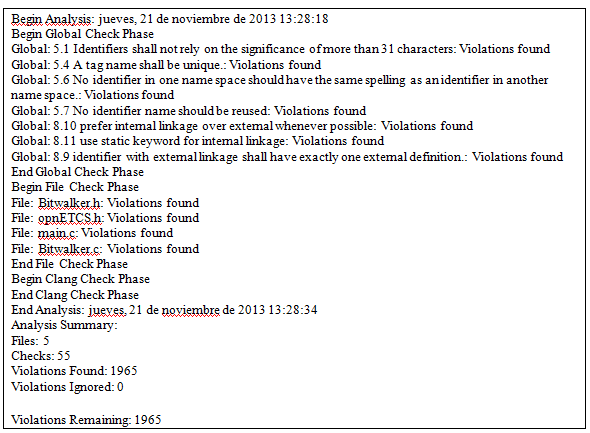
\includegraphics{./figures/understand.png}
\caption{MISRA-C Rules results}
\end{figure}

The files into the violations are found are listed in the below table.

{\footnotesize\sffamily\centering
  \begin{longtable}{||p{.15\textwidth}|p{.8\textwidth}||}
  \caption{Ubication of MISRA Violations}\\
    \hline\hline
    \textbf{MISRA Rule} & \textbf{Files} \\
    \hline\hline
    \endhead
    \hline\hline
    \endfoot
    \textbf{Global 5.1}
& Bitwalker.c/opnETCS.h/opnETCS\_Decoder.h
    \\
    \hline
    \textbf{Global 5.4}
& opnETCS.h
    \\
    \hline
    \textbf{Global 5.6}
& Bitwalker.c/Bitwalker.h
    \\
    \hline
    \textbf{Global 5.7}
& Bitwalker.c/Bitwalker.h/opnETCS.h
    \\
    \hline
    \textbf{Global 8.9}
& opnETCS\_Decoder.h
    \\
    \hline
    \textbf{Global 8.10}
& main.c
    \\
    \hline
    \textbf{Global 8.11}
& main.c
    \\
    \hline
\end{longtable}}

\subsection{Clang Static Analyzer tool Results}
The Clang Static Analyzer is a source code analysis tool that finds bugs in C, C++, and Objective-C programs.

The analyzer is 100\% open source and is part of the Clang project. Like the rest of Clang, the analyzer is implemented as a C++ library that can be used by other tools and applications.

With this analysis SQS has checked the following:

{\footnotesize\sffamily\centering
  \begin{longtable}{||p{.45\textwidth}|p{.5\textwidth}||}
  \caption{Aspects checked}\\
    \hline\hline
    \hline\hline
    \endhead
    \hline\hline
    \endfoot
    \textbf{core.AdjustedReturnValue}
& Check to see if the return value of a function call is different than the caller expects (e.g., from calls through function pointers).
    \\
    \hline
    \textbf{core.CallAndMessage}
& Check for logical errors for function calls and Objective-C message expressions (e.g., uninitialized arguments, null function pointers).
    \\
    \hline
    \textbf{core.DivideZero}
& Check for division by zero.
    \\
    \hline
    \textbf{core.NonNullParamChecker}
& Check for null pointers passed as arguments to a function whose arguments are known to be non-null.
    \\
    \hline
    \textbf{core.NullDereference}
& Check for dereferences of null pointers.
    \\
    \hline
    \textbf{core.StackAddressEscape}
& Check that addresses to stack memory do not escape the function.
    \\
    \hline
    \textbf{core.UndefinedBinaryOperatorResult}
& Check for undefined results of binary operators.
    \\
    \hline
    \textbf{core.VLASize}
& Check for declarations of VLA of undefined or zero size.
    \\
    \hline
    \textbf{core.builtin.BuiltinFunctions}
& Evaluate compiler built-in functions (e.g., alloca()).
    \\
    \hline
    \textbf{core.builtin.NoReturnFunctions}
& Evaluate "panic" functions that are known to not return to the caller.
    \\
    \hline
    \textbf{core.uninitialized.ArraySubscript}
& Check for uninitialized values used as array subscripts.
    \\
    \hline
    \textbf{core.uninitialized.Assign}
& Check for assigning uninitialized values.
    \\
    \hline
    \textbf{core.uninitialized.Branch}
& Check for uninitialized values used as branch conditions.
    \\
    \hline
    \textbf{core.uninitialized.CapturedBlockVariable}
& Check for blocks that capture uninitialized values.
    \\
    \hline
    \textbf{core.uninitialized.UndefReturn}
& Check for uninitialized values being returned to the caller.
    \\
    \hline
    \textbf{cplusplus.NewDelete}
& Check for double-free and use-after-free problems involving C++ delete.
    \\
    \hline
    \textbf{deadcode.DeadStores}
& Check for values stored to variables that are never read afterwards.
    \\
    \hline
    \textbf{osx.API}
& Check for proper uses of various Apple APIs.
    \\
    \hline
    \textbf{osx.SecKeychainAPI}
& Check for proper uses of Secure Keychain APIs.
    \\
    \hline
    \textbf{osx.cocoa.AtSync}
& Check for nil pointers used as mutexes for @synchronized.
    \\
    \hline
    \textbf{osx.cocoa.ClassRelease}
& Check for sending 'retain', 'release', or 'autorelease' directly to a Class.
    \\
    \hline
    \textbf{osx.cocoa.IncompatibleMethodTypes}
& Warn about Objective-C method signatures with type incompatibilities.
    \\
    \hline
    \textbf{osx.cocoa.NSAutoreleasePool}
& Warn for suboptimal uses of NSAutoreleasePool in Objective-C GC mode.
    \\
    \hline
    \textbf{osx.cocoa.NSError}
& Check usage of NSError** parameters.
    \\
    \hline
    \textbf{osx.cocoa.NilArg}
& Check for prohibited nil arguments to ObjC method calls.
    \\
    \hline
    \textbf{osx.cocoa.RetainCount}
& Check for leaks and improper reference count management.
    \\
    \hline
    \textbf{osx.cocoa.SelfInit}
& Check that 'self' is properly initialized inside an initializer method.
    \\
    \hline
    \textbf{osx.cocoa.UnusedIvars}
& Warn about private ivars that are never used.
    \\
    \hline
    \textbf{osx.cocoa.VariadicMethodTypes}
& Check for passing non-Objective-C types to variadic methods that expect only Objective-C types.
    \\
    \hline
    \textbf{osx.coreFoundation.CFError}
& Check usage of CFErrorRef* parameters.
    \\
    \hline
    \textbf{osx.coreFoundation.CFNumber}
& Check for proper uses of CFNumberCreate.
    \\
    \hline
    \textbf{osx.coreFoundation.CFRetainRelease}
& Check for null arguments to CFRetain/CFRelease/CFMakeCollectable.
    \\
    \hline
    \textbf{osx.coreFoundation.containers.OutOfBounds}
& Checks for index out-of-bounds when using 'CFArray' API.
    \\
    \hline
    \textbf{osx.coreFoundation.containers.PointerSizedValues}
& Warns if 'CFArray', 'CFDictionary', 'CFSet' are created with non-pointer-size values.
    \\
    \hline
    \textbf{security.FloatLoopCounter}
& Warn on using a floating point value as a loop counter (CERT: FLP30-C, FLP30-CPP).
    \\
    \hline
    \textbf{security.insecureAPI.UncheckedReturn}
& Warn on uses of functions whose return values must be always checked.
    \\
    \hline
    \textbf{security.insecureAPI.getpw}
& Warn on uses of the 'getpw' function.
    \\
    \hline
    \textbf{security.insecureAPI.gets}
& Warn on uses of the 'gets' function.
    \\
    \hline
    \textbf{security.insecureAPI.mkstemp}
& Warn when 'mkstemp' is passed fewer than 6 X's in the format string.
    \\
    \hline
    \textbf{security.insecureAPI.mktemp}
& Warn on uses of the 'mktemp' function.
    \\
    \hline
    \textbf{security.insecureAPI.rand}
& Warn on uses of the 'rand', 'random', and related functions.
    \\
    \hline
    \textbf{security.insecureAPI.strcpy}
& Warn on uses of the 'strcpy' and 'strcat' functions.
    \\
    \hline
    \textbf{security.insecureAPI.vfork}
& Warn on uses of the 'vfork' function.
    \\
    \hline
    \textbf{unix.API}
& Check calls to various UNIX/Posix functions.
    \\
    \hline
    \textbf{unix.Malloc}
& Check for memory leaks, double free, and use-after-free problems involving malloc.
    \\
    \hline
    \textbf{unix.MallocSizeof}
& Check for dubious malloc arguments involving sizeof.
    \\
    \hline
    \textbf{unix.MismatchedDeallocator}
& Check for mismatched deallocators (e.g. passing a pointer allocating with new to free()).
    \\
    \hline
    \textbf{unix.cstring.BadSizeArg}
& Check the size argument passed into C string functions for common erroneous patterns.
    \\
    \hline
    \textbf{unix.cstring.NullArg}
& Check for null pointers being passed as arguments to C string functions.
    \\
    \hline
\end{longtable}}

After run this analysis no violations have been found.

\begin{figure}[H]
\centering
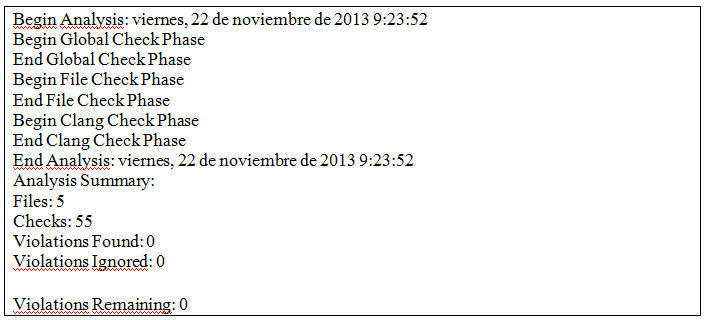
\includegraphics[scale=0.8]{./figures/clang.png}
\caption{Clang Analysis results}
\end{figure}

\subsection{CPPcheck tool Results}

Bitwalker folder has been analyzed statically by CPPcheck tool (Complying with the standard C11).
 C11 (formerly C1X) is an informal name for ISO/IEC 9899:2011, the current standard for the C programming language. It replaces the previous C standard, informally known as C99. This new version mainly standardizes features that have already been supported by common contemporary compilers, and includes a detailed memory model to better support multiple threads of execution. Due to delayed availability of conforming C99 implementations, C11 makes certain features optional, to make it easier to comply with the core language standard.
 
The results of the tool are the following:
\begin{figure}[H]
\centering
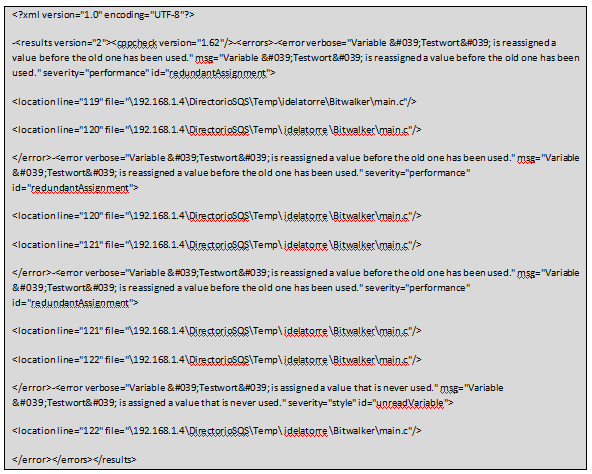
\includegraphics{./figures/cppcheck.png}
\caption{cppcheck results}
\end{figure}

\subsection{Results Comparison}
